% IEEE standard conference template; to be used with:
%   spconf.sty  - LaTeX style file, and
%   IEEEbib.bst - IEEE bibliography style file .
% --------------------------------------------------------------------------

\documentclass[letterpaper]{article}
\usepackage{spconf,amsmath,amssymb,graphicx}

% Example definitions.
% --------------------
% nice symbols for real and complex numbers
\newcommand{\R}[0]{\mathbb{R}}
\newcommand{\C}[0]{\mathbb{C}}

% bold paragraph titles
\newcommand{\mypar}[1]{{\bf #1.}}

% Title.
% ------
\title{A Descriptive Title, not too general, not too long}
%
% Single address.
% ---------------
\name{Markus P\"uschel\thanks{The author thanks Jelena Kovacevic. This paper
is a modified version of the template she used in her class.}} 
\address{Department of Computer Science\\ ETH Z\"urich\\Z\"urich, Switzerland}

% For example:
% ------------
%\address{School\\
%		 Department\\
%		 Address}
%
% Two addresses (uncomment and modify for two-address case).
% ----------------------------------------------------------
%\twoauthors
%  {A. Author-one, B. Author-two\sthanks{Thanks to XYZ agency for funding.}}
%		 {School A-B\\
%		 Department A-B\\
%		 Address A-B}
%  {C. Author-three, D. Author-four\sthanks{The fourth author performed the work
%		 while at ...}}
%		 {School C-D\\
%		 Department C-D\\
%		 Address C-D}
%

\begin{document}
%\ninept
%
\maketitle
%

The hard page limit is 6 pages in this style. Do not reduce font size
or use other tricks to squeeze. This pdf is formatted in the American letter format, so may look a bit strange when printed out.

\begin{abstract}
Describe in concise words what you do, why you do it (not necessarily
in this order), and the main result.  The abstract has to be
self-contained and readable for a person in the general area. You
should write the abstract last.

\end{abstract}

\section{Introduction}
\label{sec:introduction}
% \mypar{Motivation}
% What is online dictionary learning, why is this important.
% mention we only optimize lars?
% We optimize LARS, why we optimize LARS
% What have we optimized?
% One sentence result on how we improve it.
% Give a small description on what each section is doing
% \mypar{Related work?}


% \mypar{Online Sparse Dictionary Learning}
% % include the psuedo-code from the original paper?

Least Angle Regression (LARS) is a well-known sparse coding algorithm proposed by Bardley Efron et al\cite{Efron:04}. The algorithm is known for being less greedy and more computationally efficient to its ancestors, Forward Selection and Forward Stagewise.
One of the most common application of LARS is features selection.
Often, while training on really large dataset, the number of features within a data significantly increase the time to train the model. To decrease the number of features that represent a data while preserving the characteristics, the algorithm that is used to select the remaining features is important.

Dictionary learning, widely used in machine learning, signal processing, and image processing, is a typical case that uses feature selection algorithms.
The goal of dictionary learning is to approximate a given signal using only a few basis elements from the learned dictionary. More specifically, given a bunch of signals $Y$ in $\mathbb{R}^d$ and a dictionary $X$ in $\mathbb{R}^{d \times k}$, with k columns referred to as atoms, the algorithm is meant for finding a linear combination of most representative atoms from the dictionary.

To handle very large training sets and dynamic training data changing over time, Mairal et al. proposes an online learning algorithm for dictionary learning\cite{Mairal:2010}. In each iteration $i$ of the algorithm, sparse coding is used to compute the sparse representation $\beta_i$ of a random sample $y$ in $\mathbb{R}^d$ from a distribution $p(y)$. $\beta_i$ is then used to update the dictionary $X$.

% \mypar{Least Angle Regression (LARS)}
While feature selection algorithm like LARS are implemented to decrease the amount of time needed for training, it is obvious that the overhead of applying it should be as little as possible.
And therefore, the goal of this paper is to proposed optimization methods that are applicable to implementations of LARS and its variants, such as LASSO, and justify these optimization methods do speed up the entire procedure and enhance the performance.

In the following sections, we formally define LARS, introduce incremental Cholesky decomposition and shows a detail cost analysis on the entire procedure in Section~\ref{sec:background}.
We present the optimization we applied in Section~\ref{sec:method} and show the result in Section~\ref{sec:experiment}. At last, we summarize our work in Section~\ref{sec:conclusions}.






%  Do not start the introduction with the abstract or a slightly modified
%  version. It follows a possible structure of the introduction. 
%  Note that the structure can be modified, but the
%  content should be the same. Introduction and abstract should fill at most the first page, better less.
 
%  \mypar{Motivation} The first task is to motivate what you do.  You can
%  start general and zoom in one the specific problem you consider.  In
%  the process you should have explained to the reader: what you are doing,
%  why you are doing, why it is important (order is usually reversed).
 
%  For example, if my result is the fastest DFT implementation ever, one
%  could roughly go as follows. First explain why the DFT is important
%  (used everywhere with a few examples) and why performance matters (large datasets,
%  realtime). Then explain that fast implementations are very hard and
%  expensive to get (memory hierarchy, vector, parallel). 
 
%  Now you state what you do in this paper. In our example: 
%  presenting a DFT implementation that is
%  faster for some sizes than all the other ones.
 
%  \mypar{Related work} Next, you have to give a brief overview of
%  related work. For a paper like this, anywhere between 2 and 8
%  references. Briefly explain what they do. In the end contrast to what
%  you do to make now precisely clear what your contribution is.


\section{Background: Whatever the Background is}
\label{sec:background}

In this section, we first introduce a formal representation of LARS and the algorithm that is implemented to solve the formulas.
We then introduce Incremental Cholesky decomposition in Section~\ref{ssec:cholesky} and formulate how we calculate the cost of the program in Section~\ref{ssec:cost-analysis} and show the exact number of operations throughout the whole program in Table~\ref{tab:cost}.

\subsection{A Formal Definition of LARS}
An L1-regularized linear regression problem is described as follows:
$$
min_\beta{||y-X\beta||^2_2} \ s.t\ ||\beta||_1 \leq l
$$
And the dual form of the problem that LARS solves:
$$
min_\beta{||y-X\beta||^2_2} + \lambda||\beta||_1
$$

A more formal representation of how LARS produces a piece-wise linear solution path is described in Algorithm~\ref{alg:lars}.
In the beginning of the algorithm, the current residual is equal to the input $y$. The correlation is initialized at line~\ref{alg:lars:initailize_correlation}.
In each iteration, the correlation is updated and the most correlated basis to current residual is added into the active set $A$ as shown in line~\ref{alg:lars:get_active_idx} - \ref{alg:lars:get_active_idx_end}.
The unit vector of the equiangular direction, $u_A$, is computed in line~\ref{alg:lars:cholesky} - \ref{alg:lars:get_a}, and the distance to walk is computed at line~\ref{alg:lars:get_gamma}.
The current approximation of $y$ is then update at line~\ref{alg:lars:update_beta}.
The \texttt{while} loop continues until the $\hat{\lambda}$, computed at line~\ref{alg:lars:compute_lambda} is greater than the given parameter $\lambda$.


% Insert the algorithm
\begin{algorithm}
	\caption{Compute sum of integers in array}
	\label{alg:lars}
	\begin{algorithmic}[1]
		\Procedure{LARS}{$X, y, \lambda$}
		    \State $\hat{c} = X^T y$, $\hat{\beta} \gets 0$ \label{alg:lars:initailize_correlation}
		    \While {\textsc{Compute\_$\lambda$()} $< \lambda$ }
		      % Get_active_idx
		      \State $\hat{c} \gets \hat{c} - X^T \hat{\beta}$ \label{alg:lars:get_active_idx}
		      \State $\hat{C} \gets \max_j{|\hat{c}_j|}$
		      , $A \gets \{j, |\hat{c}_j| = \hat{C} \}$
		      \State $s_A \gets \{sign(\hat{c}_j), j \in A\}$ \label{alg:lars:get_active_idx_end}
		      
		      % Cholesky
		      \State $G_A \gets X_A^T X_A$ \label{alg:lars:cholesky}
		      \State $w_A \gets G_A^{-1} s_A$
		      \label{alg:lars:inversion}
		      \State $A_A \gets \sqrt{1_A^T w_A}$ \label{alg:lars:cholesky_end}
		      
		      % Get_U
		      \State $u_A \gets A_A X_A w_A$ \label{alg:lars:get_u}
		      
		      % Get_A
		      \State $a \gets X^T u_A$ \label{alg:lars:get_a}

		      % Get_gamma
		      \State $\hat{\gamma} = \min_{j \in A^c}^+ \Big\{ \frac{\hat{C} - \hat{c_j}}{A_A - a_j},  \frac{\hat{C} + \hat{c_j}}{A_A + a_j}\Big\}$ \label{alg:lars:get_gamma}
		      
		      % Update_beta
		      \State $\hat{\beta} \gets \hat{\beta} + \hat{\gamma} u_A$ \label{alg:lars:update_beta}
		    
		    \EndWhile
            \State Return $\hat{\beta}$
		\EndProcedure
		
		\Procedure{Compute\_$\lambda$}{}\label{alg:lars:compute_lambda}
		    \State $\Lambda = X_A^T ( X_A \hat{\beta} - y)$
    		\State Return $\max_{\lambda_i \in \Lambda} \big\{ |\lambda_i| \big\}$ 
		\EndProcedure
	\end{algorithmic}
\end{algorithm}


\subsection{Incremental Cholesky}
\label{ssec:cholesky}
%\mypar{baseline implementation}
In order to solve $w_A$, the weighting function that composes the new direction as shown in line~\ref{alg:lars:inversion} of the Algorithm~\ref{alg:lars}, we have to calculate the inverse of the correlation matrix of the active basis. Throughout each iteration, one new basis will be added into the active basis. Instead of recalculating the inverse, which is $O(n^3)$ in complexity, in every iteration, we use incremental cholesky, which is $O(N^2)$ in complexity, that updates the triangular solver according to the newly added basis in each iteration.

We separate the baseline version of implementation that solves $w_A = G_A^{-1} s_A$ into two parts: \textit{update cholesky solver} and \textit{backsolve the target}.

\mypar{Update cholesky solver}
Suppose we have a correlation matrix $X_{A_{t-1}}^T X_{A_{t-1}}$, in iteration $t$, to update the correlation matrix with the new basis $v$, we only add a new column and a new row to the previous correlation matrix, getting the new correlation matrix:
\[
G_{A_t} = 
\begin{bmatrix}
X_{A_{t-1}}^T X_{A_{t-1}}   &   X_{A_{t-1}}^T v \\
v^T X_{A_{t-1}}             &   \sqrt{v^T v}
\end{bmatrix}
\].
We then update the lower triangle of $G_A$ with:
\[
L_t = 
\begin{bmatrix}
L_{t-1}   &    0 \\
v^T X_{A_{t-1}} (L_{t-1}^{-1})^T  &  \sqrt{v^T v - |v^T X_A (L_{t-1}^-1)^T | ^2}
\end{bmatrix}
\]
To compute $v^T X_{A_{t-1}} (L_{t-1}^{-1})^T$, we solve $w$ for
$$
L_{t-1} w = X_{A_{t-1}} v
$$ with Gaussian elimination. 

\mypar{backsolve the target}
Inverting correlation matrix $G_{A_t}$ is inverting the corresponding Cholesky decomposition $LL^T$, which can be done by solving a lower triangular system and a upper triangular system sequentially. 



\subsection{Cost Analysis}
\label{ssec:cost-analysis}
% Define cost measure
Each math function (add, mult, div, sqrt, etc.) is associated with a specific number of floating point operations, which is derived from the proportion of its throughput to the throughput of floating point addition. For example, a division of two doubles counts as 16 floating point operations, because the throughput of  \texttt{\_mm256\_div\_pd} is $1/8$ according to Intel Intrinsics Guide \cite{Intrinsics} while the throughput of \texttt{\_mm256\_add\_pd} is two. The relative floating point operation counts of all math functions used in the algorithm is listed in Table~\ref{tab:flop_def}.
 
\begin{table}
\centering
\begin{tabular}{|c||c|c|c|c|c|c|c|}
\hline
operation & cmp & add & mul & fma & div & sqrt & abs \\ \hline
flop count & 1 & 1 & 1 & 1 & 16 & 24 & 1.5 \\ \hline
\end{tabular}
\caption{Relative flop count of operations.}
\label{tab:flop_def}
\end{table}

%% Description for the table.
Since we are solving sparse and overcomplete representations of input, the dictionary size $k$ is usually larger than the signal dimension $d$. The number of iterations in LARS depends on the regularization parameter $\lambda$ and the values of the target signal. For simplicity of analysis, we set $k = 2d$ and $\lambda = 0$, so that the algorithm always ends in $d$ iterations. 

For optimization purposes, we counted the exact floating point operations within different parts of the algorithm LARS as shown in Table~\ref{tab:cost}. With Table~\ref{tab:flop_def} and Table~\ref{tab:cost}, we can calculate the approximate floating point operation counts of each code segment.


\begin{table*}[ht!]
\centering
\begin{tabular}{|c || c | c | c | c | c | c | c | c |}
\hline
 Code Segment & Line & cmp & add & mul & fma & div & sqrt & abs \\
\hline\hline
\textsc{Init\_Correlation} & 2 & 0 & 0 & 0 & $2D^2$ & 0 & 0 & 0 \\ 
\textsc{Find\_Active\_Idx} & 4-6 & $7D^2+D$ & 0 & 0 & 0 & 0 & 0 & $\frac{D(D+1)}{2}$ \\
\textsc{Fused\_Cholesky} & 7-9 & $D$ & $\frac{D(D+1)}{2}$ & 0 & $\frac{D(D+1)(8D-2)}{6}$ & $\frac{D(D+1)}{2}$ & $2D$ & $\frac{D(D+1)}{2}$ \\
\textsc{Compute\_U} & 10 & 0 & 0 & $\frac{D(D+1)}{2}$ & $\frac{D^2(D+1)}{2}$ & 0 & 0 & 0  \\
\textsc{Compute\_A} & 11 & 0 & 0 & 0 & $2D^3$ & 0 & 0 & 0  \\
\textsc{Compute\_$\gamma$} & 12 & $4D^2+3D$ & $2D^2+2D$ & 0 & 0 & $D^2+2D$ & 0 & 0  \\
\textsc{Update\_$\beta$} & 13 & 0 & 0 & 0 & $\frac{D(D+1)}{2}$ & 0 & 0 & 0  \\
\textsc{Compute\_$\lambda$} & 18 & $2D^2$ & 0 & 0 & $\frac{D^2(D+3)}{2}$ & 0 & 0 & $2D^2$  \\
\hline
\textsc{Total} & * & $13D^2+4D$ & $\frac{5D(D+1)}{2}$ & $\frac{D(D+1)}{2}$ & $\frac{D(29D^2+42D+1)}{6}$ & $\frac{D(3D+5)}{2}$ & $2D$ & $D(3D+1)$  \\
\hline
\end{tabular}
\caption{Cost analysis on each code segments of Algorithm~\ref{alg:lars}. $D$ is the dimension of the target signal.}
\label{tab:cost}
\end{table*}

% Asymptotic complexity






%  Give a short, self-contained summary of necessary
%  background information. For example, assume you present an
%  implementation of FFT algorithms. You could organize into DFT
%  definition, FFTs considered, and cost analysis. The goal of the
%  background section is to make the paper self-contained for an audience
%  as large as possible. As in every section
%  you start with a very brief overview of the section. Here it could be as follows: In this section 
%  we formally define the discrete Fourier transform, introduce the algorithms we use
%  and perform a cost analysis.
%  
%  \mypar{Discrete Fourier Transform}
%  Precisely define the transform so I understand it even if I have never
%  seen it before.
%  
%  \mypar{Fast Fourier Transforms}
%  Explain the algorithm you use.
%  
%  \mypar{Cost Analysis}
%  First define you cost measure (what you count) and then compute the
%  cost. Ideally precisely, at least asymptotically. In the latter case you will 
%  need to instrument your code to count
%  the operations so you can create a performance plot.
%  
%  Also state what is
%  known about the complexity (asymptotic usually) 
%  about your problem (including citations).
%  
%  Don't talk about "the complexity of the algorithm.'' It's incorrect,
%  remember (Lecture 2)?

\section{Your Proposed Method}
\label{sec:method}
Now comes the ``beef'' of the paper, where you explain what you
did. Again, organize it in paragraphs with titles. As in every section
you start with a very brief overview of the section.

For this class, explain all the optimizations you performed. This mean, you first very briefly
explain the baseline implementation, then go through locality and other optimizations, and finally SSE (every project will be slightly different of course). Show or mention relevant analysis or assumptions. A few examples: 1) Profiling may lead you to optimize one part first; 2) bandwidth plus data transfer analysis may show that it is memory bound; 3) it may be too hard to implement the algorithm in full generality: make assumptions and state them (e.g., we assume $n$ is divisible by 4; or, we consider only one type of input image); 4) explain how certain data accesses have poor locality. Generally, any type of analysis adds value to your work.

As important as the final results is to show that you took a structured, organized approach to the optimization and that you explain why you did what you did.

Mention and cite any external resources including library or other code.

Good visuals or even brief code snippets to illustrate what you did are good. Pasting large amounts of code to fill the space is not good.



\section{Experimental Results}
\label{sec:experiment}

In this section, we evaluate the optimization strategies proposed in Section~\ref{sec:method}.
We detail the settings of the machine that we performed our test on, and then
present the results of our optimization.

\subsection{Experimental setup}

The program is implemented in double-precision floating points due to precision problems.
All performance experiments are conducted on Red Hat Enterprise Linux 7 running on a machine with the specifications as shown in Table~\ref{tab:cpu-info}.
% CPU:Intel i7-6700 CPU @ 3.40GHz (skylake)\\
% L1 data cache,    	line size 64,  8-ways,	64 sets, size 32k\\
% L1 instruction cache, line size 64,  8-ways,	64 sets, size 32k\\
% L2 unified cache, 	line size 64,  4-ways,  1024 sets, size 256k\\
% L3 unified cache, 	line size 64, 16-ways,  8192 sets, size 8192k
% \lc{use table for this?}
\begin{table}
\begin{center}
\begin{tabular}{ | c | c | c | c | c | }
%  \hline
%  \multicolumn{5}{|l|}{Intel i7-6700 CPU @ 3.40GHz (skylake)}\\
%  \hline
 \hline
     & line size & \# ways & \# sets  & size\\  \hline
 L1 data cache        & 64 &  8 &   64 & 32K \\  \hline
 L1 instruction cache & 64 &  8 &   64 & 32K \\  \hline
 L2 unified cache     & 64 &  4 & 1024 & 256K \\ \hline
 L3 unified cache     & 64 & 16 & 8192 & 8M \\  
 \hline
\end{tabular}
\caption{Specification of Intel i7-6700 CPU @ 3.40GHz (skylake).\cite{Intel_i7-6700}}
\label{tab:cpu-info}
\end{center}
\end{table}

The maximal memory bandwidth advertised is 34.1 GB/s, but in practice it's guaranteed to be less than that. We hence use \textit{bandwidth}\cite{bandwidth} to measure sustained memory bandwidth for different access patterns. From the benchmark result in Figure~\ref{fig:mem-bw}, the memory bandwidth of random read and write are 21.2 GB/s and 3.10 GB/s respectively for data of size 512 MB. We thus take these two bandwidth as the memory bounds as the upper-bound of the memory in our roofline model.

The intersection of the peak performance bound and the memory bandwidth bound is at $I = \pi/\beta$. For scalar code, the intersection is between 0.64 and 4.38 flop/byte. As for vectorized code, the intersection is between 2.56 and 17.55 flop/byte.

We use Linux \texttt{perf} command \cite{perf} to monitor hardware event such as cache miss and number of load/store invocation. The number of last-level cache (LLC) miss can give us an idea of the data traffic between CPU and main memory.

%% should we talk about how we segment our code here?

The compilers we use for all the statistics in this paper are Intel C/C++ Compiler (\textit{icc 14.0.0.20131008}) For the baseline, the compiler flag is \textit{-O3 -ansi-alias -no-vec -unroll=0}. As for the our best optimized version, we set the flag to \textit{-O3 -std=c++11 -xHost -ansi-alias -unroll=4 -march=core-avx2 -auto-ilp32}.

% \begin{center}
% \begin{tabular}{ | c | c | c | }\label{tab:cpu-info}
%  \hline
%  cell1 & cell2 & cell3 \\
%  \hline
%  cell4 & cell5 & cell6 \\  
%  cell7 & cell8 & cell9 \\
%  \hline
% \end{tabular}
% \caption{}
% \end{center}


%% Results

\subsection{Results}

Figure~\ref{fig:performance} shows the performance gain from all the optimization techniques we adopt. With proper unrolling and vectorize compiler flags, the performance is improved by 3.7 times, from 0.57 flops/cycle to 2.12 flops/cycle. With all the other approaches mentioned in Section~\ref{sec:method} that improves data locality and reduce computation, we further enhanced the performance to 4.10 flops/cycle, which gives us 7.2 times speed-up in total comparing to the baseline version. The run time proportion after optimization is shown in Figure~\ref{fig:pie_after} 

\begin{figure}
\centering
  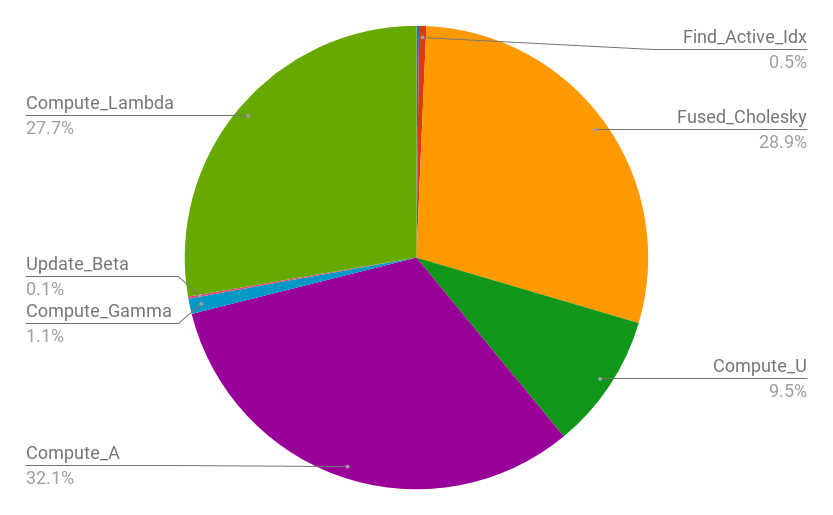
\includegraphics[scale=0.26]{./pic/pie_after.png}
  \caption{Run time after optimization}
  \label{fig:pie_after}
\end{figure}

\begin{figure}[h]
\centering
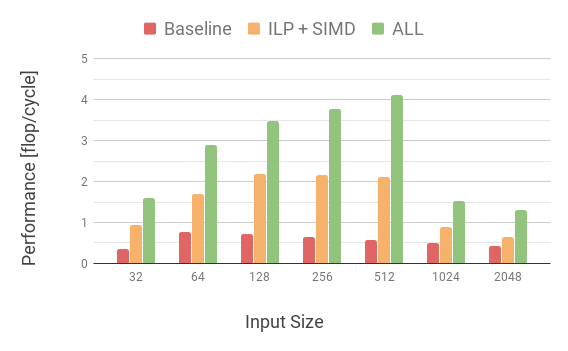
\includegraphics[width=0.5\textwidth]{./pic/performance.png}
\caption{Performance Comparison. \textsc{Baseline} is compiled w/o optimization flags, \textsc{ILP+SIMD} is baselin compiled with optimization falgs and \textsc{ALL} is our final optimized version.}
\label{fig:performance}
\end{figure}


As the input size increases, the overhead of optimization, such as extra branches for corner case of blocking and unrolling, become insignificant as the benefit grows faster. On the other hand, the performance and the speed-up gain drop dramatically on input sizes larger than 1024. One reason might be that for input size of 1024, the allocated memory space exceed the 8MB physical memory space. Then the run time is dominated by the access time of hard disk.


\begin{figure*}
\centering
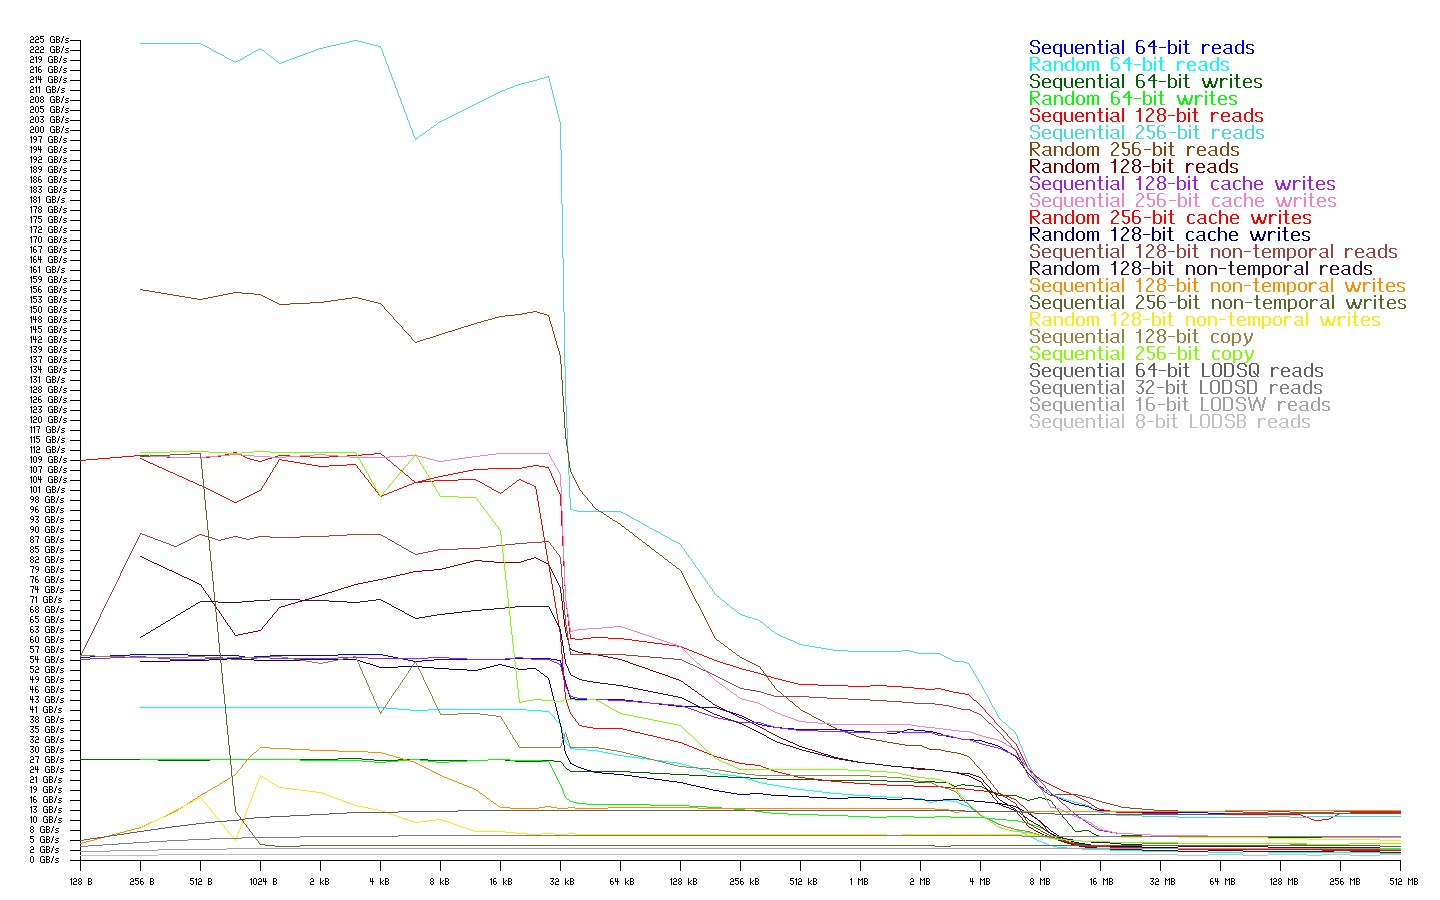
\includegraphics[scale=0.18]{./pic/bandwidth.jpg}
\caption{Measured memory bandwidth}
\label{fig:mem-bw}
\end{figure*}

The memory traffic is estimated as: 
$$
\# LLC\ misses \cdot LLC\ line\ size
$$
As argued by Georg Ofenbeck et al.\cite{ofenbeck2014applying} the actual traffic might be more than, even twice, the amount of observed LLC cache misses, depending on caching mechanism. Even though, it's still good upper bound of of memory traffic. Combining the measured memory traffic, measured run time cycles, and calculated floating point operation counts, we draw the roofline plot and examine the limitation of optimizing this algorithm.

\begin{figure}[h]
\centering
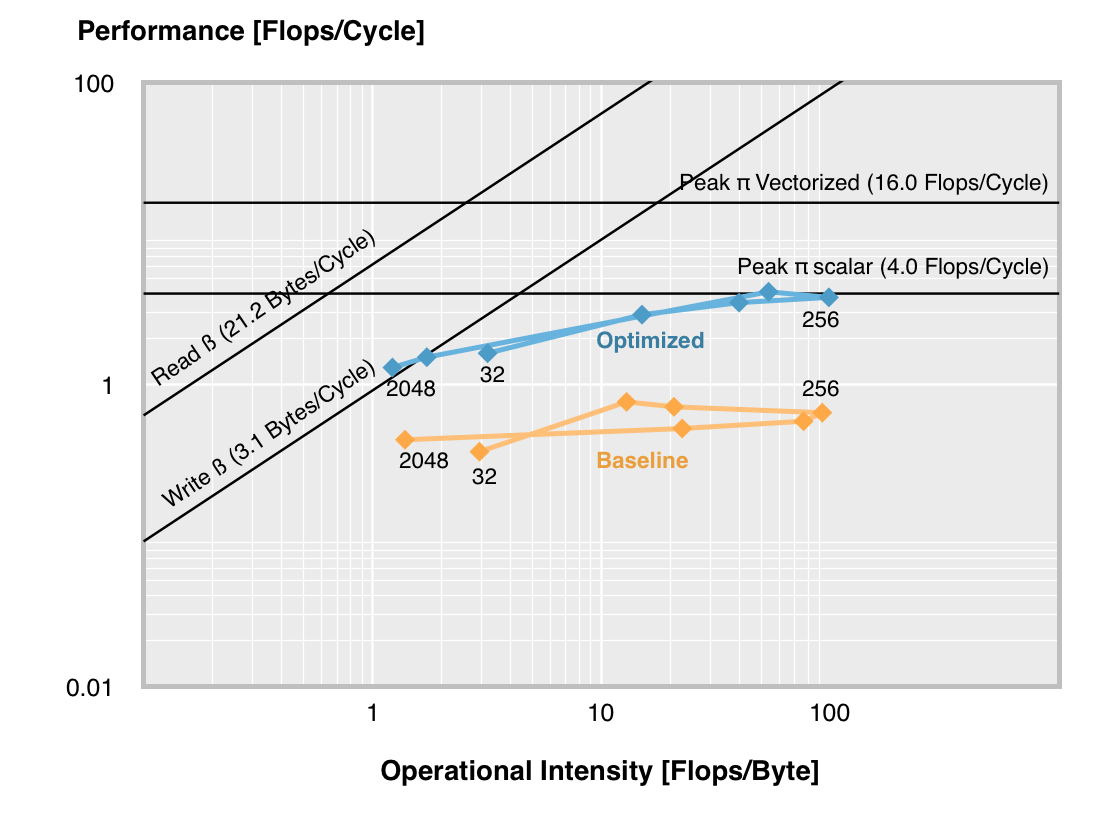
\includegraphics[width=0.5\textwidth]{./pic/roofline.png}
\caption{Roofline plot of baseline and optimized program.}
\label{fig:roofline}
\end{figure}

From the roofline plot in Figure~\ref{fig:roofline}, we know that the larger the input size is (larger than 256), the more likely the algorithm is memory bounded.





% Here you evaluate your work using experiments. You start again with a
% very short summary of the section. The typical structure follows.

% \mypar{Experimental setup} Specify the platform (processor, frequency, cache sizes)
% as well as the compiler, version, and flags used. I strongly recommend that you 
% play with optimization flags and consider also icc for additional potential speedup.

% Then explain what input you used and what range of sizes. The idea is to give 
% enough information so the experiments are reproducible by somebody else on his or her code.

% \mypar{Flags}
% -fma or/Qfma. If the instructions exist on the target processor, the compiler generates fused multiply-add (FMA) instructions.

% \mypar{Results}
% Next divide the experiments into classes, one paragraph for each. In the simplest
% case you have one plot that has the size on the x-axis and the performance on the
% y-axis. The plot will contain several lines, one for each relevant code version.
% Discuss the plot and extract the overall performance gain from baseline to best 
% code. Also state the percentage of peak performance for the best code. Note that
% the peak may change depending on the situation. For example, if you only do 
% additions it would be 12 Gflop/s
% on one core with 3 Ghz and SSE and single precision floating point.

% Do not put two performance lines into the same plot if the operations count 
% changed significantly (that's apples and oranges). In that case first perform 
% the optimizations that reduce op count and report the runtime gain in a plot. 
% Then continue to optimize the best version and show performance plots.

% {\bf You should}
% \begin{itemize}
% \item Follow the guide to benchmarking presented in class, in particular
% \item very readable, attractive plots (do 1 column, not 2 column plots
% for this class), proper readable font size. An example is below (of course you 
% can have a different style),
% \item every plot answers a question, which you pose and extract the
% answer from the plot in its discussion
% \end{itemize}
% Every plot should be discussed (what does it show, which statements do
% you extract).

\section{Conclusions}
\label{sec:conclusions}
Here you need to briefly summarize what you did and why this is
important. {\em Do not take the abstract} and put it in the past
tense. Remember, now the reader has (hopefully) read the paper, so it
is a very different situation from the abstract. Try to highlight
important results and say the things you really want to get across
(e.g., the results show that we are within 2x of the optimal performance ... 
Even though we only considered the DFT, our optimization
techniques should be also applicable ....) You can also formulate next
steps if you want. Be brief.

\section{Further comments}

Here we provide some further tips.

\mypar{Further general guidelines}

\begin{itemize}
\item For short papers, to save space, I use paragraph titles instead of
subsections, as shown in the introduction.

\item It is generally a good idea to break sections into such smaller
units for readability and since it helps you to (visually) structure the story.

\item The above section titles should be adapted to more precisely
reflect what you do.

\item Each section should be started with a very
short summary of what the reader can expect in this section. Nothing
more awkward as when the story starts and one does not know what the
direction is or the goal.

\item Make sure you define every acronym you use, no matter how
convinced you are the reader knows it.

\item Always spell-check before you submit (to me in this case).

\item Be picky. When writing a paper you should always strive for very
high quality. Many people may read it and the quality makes a big difference.
In this class, the quality is part of the grade.

\item Books helping you to write better: \cite{Higham:98} and \cite{Strunk:00}.

\item Conversion to pdf (latex users only): 

dvips -o conference.ps -t letter -Ppdf -G0 conference.dvi

and then

ps2pdf conference.ps
\end{itemize}

\mypar{Graphics} For plots that are not images {\em never} generate (even as intermediate step)
jpeg, gif, bmp, tif. Use eps, which means encapsulate postscript, os pdf. This way it is
scalable since it is a vector graphic description of your graph. E.g.,
from Matlab, you can export to eps or pdf.

Here is an example of how to get a plot into latex
(Fig.~\ref{fftperf}). Note that the text should not be any smaller than shown.

\begin{figure}\centering
  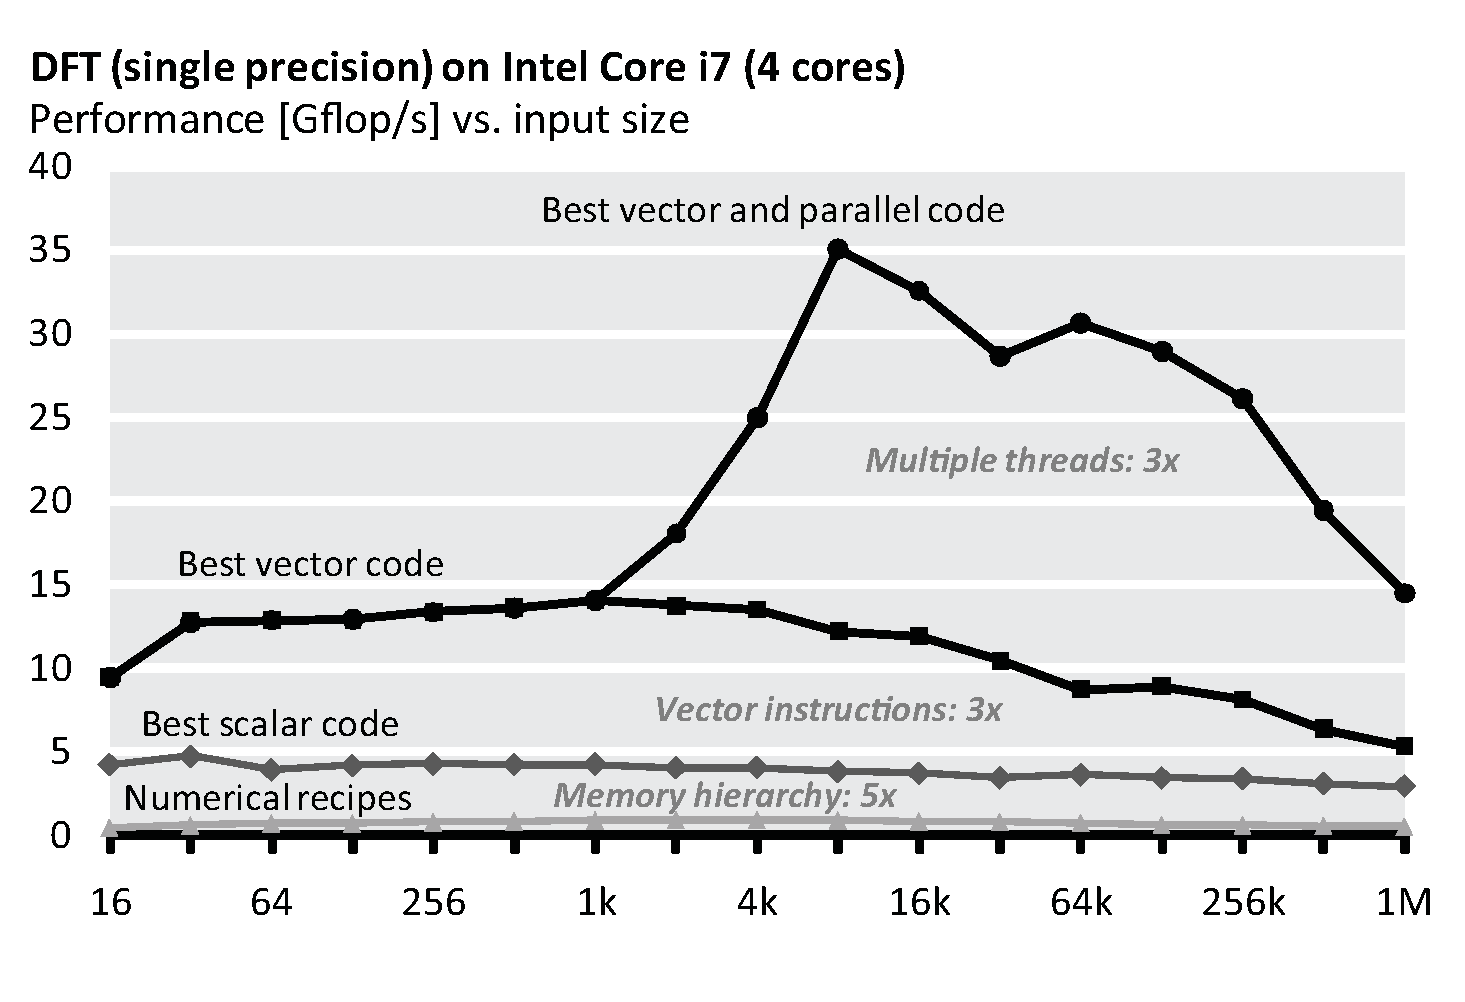
\includegraphics[scale=0.33]{dft-performance.eps}
  \caption{Performance of four single precision implementations of the
  discrete Fourier transform. The operations count is roughly the
  same. {\em The labels in this plot are too small.}\label{fftperf}}
\end{figure}




% References should be produced using the bibtex program from suitable
% BiBTeX files (here: bibl_conf). The IEEEbib.bst bibliography
% style file from IEEE produces unsorted bibliography list.
% -------------------------------------------------------------------------
\bibliographystyle{IEEEbib}
\bibliography{bibl_conf}

\end{document}

